%---------------------------------------------------------------------      
    \section*{Extra}
	%------------------------------ SLIDE ---------------------------------------
    \begin{frame}{} % cada entorno frame es una diapositiva
        \justifying % para justificar el texto, siempre al inicio de cada frame
        % Añade espacio para mover el bloque hacia arriba
        % Añade espacio para mover el bloque hacia arriba
        \vspace*{-0.5cm} % Ajusta este valor según sea necesario
        
        % Define los colores del bloque
        \definecolor{custombgcolor2}{RGB}{155, 134, 189} % Color de fondo
        \definecolor{customfgcolor2}{RGB}{0, 0, 0} % Color del texto

        % Cuadro sin bordes redondeados, con colores personalizados
        \begin{tcolorbox}[colback=custombgcolor2, coltext=customfgcolor2,
                      colframe=custombgcolor2, % Color del borde
                      width=\textwidth,       % Ancho del cuadro
                      boxrule=1pt,            % Grosor del borde
                      top=1mm, bottom=1mm,     % Espacio superior e inferior
                      sharp corners=all,     % Bordes sin redondear
                      halign=center,         % Alineación horizontal
                      valign=center,         % Alineación vertical
                      ]
        % Texto dentro del cuadro
        \textbf{Mecanismos \kern-0.9em de \kern-0.9em aceleración}
        \end{tcolorbox}

        \begin{columns}
            \begin{column}{0.45\textwidth} % Columna izquierda para la lista
            		\textbf{\small Mecanismo de \emph{Fermi} de segundo orden:}
                \begin{itemize}
                    \item Nubes de plasma en movimiento.
                    \item Puede acelerar partículas mediante la transferencia de energía cinética.
                    \item La energía se expresa como: \[E_{n} = E_{0} \left(1 + \frac{4}{3} \beta^{2}\right)^{n}\]
                    \item $\beta = v/c$.
                \end{itemize}
            \end{column}

            \begin{column}{0.4\textwidth} % Columna derecha para la imagen
                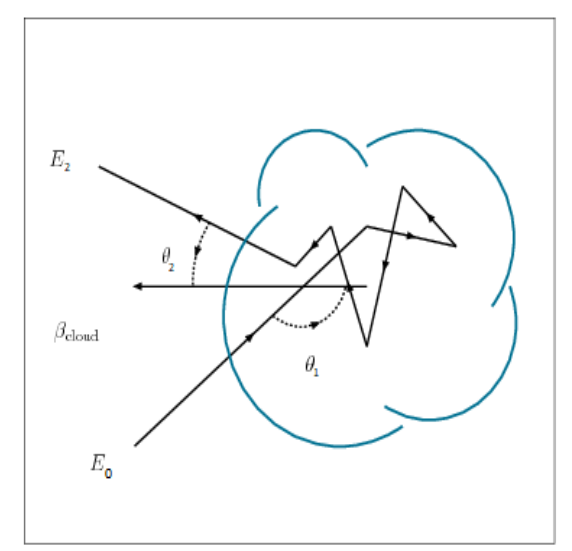
\includegraphics[width=1.16\textwidth]{Figures/fermisecondorder.png}
            \end{column}
        \end{columns}
    \end{frame}
    
	%------------------------------ SLIDE ---------------------------------------
    \begin{frame}{} % cada entorno frame es una diapositiva
        \justifying % para justificar el texto, siempre al inicio de cada frame
        % Añade espacio para mover el bloque hacia arriba
        % Añade espacio para mover el bloque hacia arriba

        \begin{columns}
            \begin{column}{0.45\textwidth} % Columna izquierda para la lista
            		\textbf{\small Mecanismo de \emph{Fermi} de primer orden:}
                \begin{itemize}
                    \item Frentes de choque (e.g. supernovas).
                    \item La energía se expresa como: \[E_{n} = E_{0} \left(1 + \frac{4}{3} \beta\right)^{n}\]
                    \item Es el mecanismo más eficiente.
                    \item Reproduce una ley de potencia con $\alpha \simeq 2$.
                \end{itemize}
            \end{column}

            \begin{column}{0.4\textwidth} % Columna derecha para la imagen
                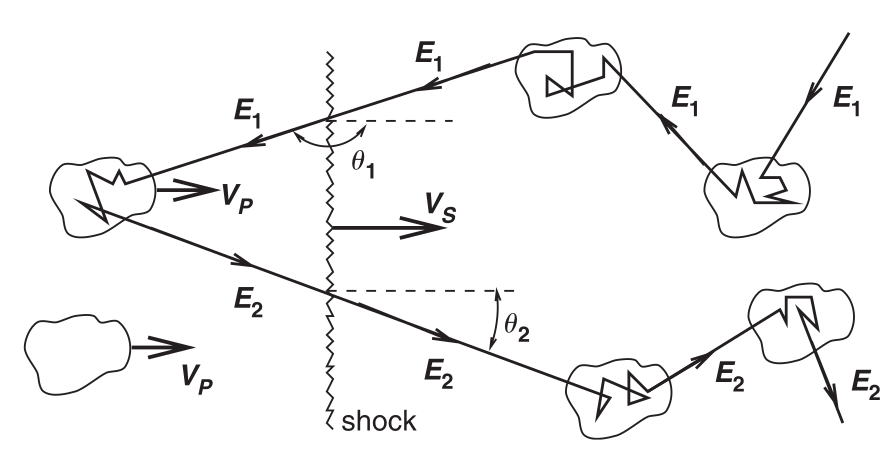
\includegraphics[width=1.16\textwidth]{Figures/fermifirstorder.png}
            \end{column}
        \end{columns}
    \end{frame}